\chapter{Sistema de Autenticaci\'on}

\section{Arquitectura General}

El sistema de autenticaci\'on utiliza \textbf{NextAuth v5} (beta 31) con
\textbf{proveedor de credenciales} (email y contrase\~na) y \textbf{estrategia
de sesi\'on JWT}. Los roles de usuario se inyectan en el token JWT y se
utilizan para control de acceso tanto en el servidor como en el cliente.

\section{Configuraci\'on de NextAuth}

\subsection{auth.config.ts --- Configuraci\'on Base}

El archivo \texttt{lib/auth.config.ts} define la configuraci\'on base de
NextAuth, incluyendo la extensi\'on de tipos de TypeScript:

\begin{lstlisting}[style=typescript, caption=auth.config.ts - Extension de tipos y configuracion base]
// Extension de tipos para incluir role y clinicId
declare module 'next-auth' {
  interface User {
    role: 'super_admin' | 'admin' | 'veterinarian'
        | 'technician' | 'receptionist';
    clinicId: number;
  }
  interface Session {
    user: {
      id: string;
      role: UserRole;
      name: string;
      email: string;
      clinicId: number;
    };
  }
}

export const authConfig: NextAuthConfig = {
  providers: [],
  pages: {
    signIn: '/auth/login',
  },
  session: { strategy: 'jwt' },
  callbacks: {
    async jwt({ token, user }) {
      if (user) {
        (token as any).role = user.role;
        (token as any).id = user.id;
        (token as any).clinicId = user.clinicId;
      }
      return token;
    },
    async session({ session, token }) {
      if (session.user) {
        (session.user as any).role = (token as any).role;
        (session.user as any).id = (token as any).id;
        (session.user as any).clinicId = (token as any).clinicId;
      }
      return session;
    },
  },
};
\end{lstlisting}

\subsection{auth.ts --- Instancia de NextAuth}

\begin{lstlisting}[style=typescript, caption=auth.ts - Proveedor de credenciales]
export const { handlers, signIn, signOut, auth } = NextAuth({
  ...authConfig,
  secret: process.env.AUTH_SECRET,
  providers: [
    Credentials({
      name: 'credentials',
      credentials: {
        email: { label: 'Email', type: 'email' },
        password: { label: 'Password', type: 'password' },
      },
      async authorize(credentials) {
        if (!credentials?.email || !credentials?.password)
          return null;

        const email = credentials.email as string;
        const password = credentials.password as string;

        try {
          const user = await db
            .select()
            .from(schema.users)
            .where(eq(schema.users.email, email))
            .then((rows) => rows[0]);

          if (!user || !user.active) return null;

          const isValid = await compare(password, user.passwordHash);
          if (!isValid) return null;

          return {
            id: String(user.id),
            email: user.email,
            name: `${user.firstName} ${user.lastName}`,
            role: user.role as UserRole,
            clinicId: user.clinicId,
          };
        } catch (err) {
          console.error('[AUTH DB ERROR]', err);
          return null;
        }
      },
    }),
  ],
});
\end{lstlisting}

\section{Middleware de Protecci\'on}

El middleware de Next.js protege las rutas del dashboard:

\begin{lstlisting}[style=typescript, caption=middleware.ts - Proteccion de rutas]
import NextAuth from 'next-auth';
import { authConfig } from '@/lib/auth.config';
import { NextResponse } from 'next/server';

const { auth } = NextAuth(authConfig);

const publicRoutes = ['/auth/login', '/auth/register'];

export default auth((req) => {
  const { nextUrl } = req;
  const session = req.auth;

  if (!session) {
    if (publicRoutes.some((route) =>
        nextUrl.pathname.startsWith(route))) {
      return NextResponse.next();  // Ruta publica
    }
    return NextResponse.redirect(
      new URL('/auth/login', nextUrl)
    );
  }

  // Usuario autenticado en ruta publica -> redirige a dashboard
  if (!publicRoutes.some((route) =>
      nextUrl.pathname.startsWith(route))) {
    return NextResponse.next();
  }

  return NextResponse.redirect(new URL('/', nextUrl));
});

export const config = {
  matcher: ['/((?!api|_next/static|_next/image|favicon.ico).*)'],
};
\end{lstlisting}

\section{Flujo de Autenticaci\'on}

\subsection{Login}

La p\'agina \texttt{/auth/login} es un componente cliente que:

\begin{enumerate}
    \item Presenta un formulario con email y contrase\~na.
    \item Env\'{\i}a las credenciales mediante \texttt{signIn('credentials',
          \{...\})}.
    \item Muestra errores gen\'ericos ``Credenciales inv\'alidas''.
    \item Redirige al dashboard tras autenticaci\'on exitosa.
    \item Incluye animaciones con Framer Motion (mascotas flotantes,
          transiciones, gradientes animados).
\end{enumerate}

\subsection{Registro}

La p\'agina \texttt{/auth/register} y la API \texttt{POST /api/auth/register}:

\begin{enumerate}
    \item Validan campos obligatorios (nombre, apellido, email, contrase\~na).
    \item Verifican que el email no est\'e registrado.
    \item Hashean la contrase\~na con \textbf{bcryptjs} (12 rondas).
    \item Asignan el usuario a la cl\'{\i}nica activa por defecto.
    \item Crean el usuario con rol \texttt{receptionist} por defecto.
    \item Retornan error 500 en caso de fallo interno.
\end{enumerate}

\section{Proveedores del Lado del Cliente}

La sesi\'on se propaga mediante \texttt{SessionProvider} de NextAuth:

\begin{lstlisting}[style=typescript, caption=providers.tsx]
'use client';

import { SessionProvider } from 'next-auth/react';

export function Providers({ children }: { children: React.ReactNode }) {
  return <SessionProvider>{children}</SessionProvider>;
}
\end{lstlisting}

El \texttt{SessionProvider} se incluye en el \texttt{RootLayout}:

\begin{lstlisting}[style=typescript, caption=RootLayout]
export default function RootLayout({
  children
}: { children: React.ReactNode }) {
  return (
    <html lang="es" suppressHydrationWarning>
      <body>
        <ThemeProvider attribute="class" defaultTheme="system"
                      enableSystem disableTransitionOnChange>
          <Providers>{children}</Providers>
        </ThemeProvider>
      </body>
    </html>
  );
}
\end{lstlisting}

\section{Uso de la Sesion en Componentes}

\subsection{Navbar --- Informacion del Usuario}

La Navbar muestra el nombre del usuario autenticado, iniciales en el avatar
y men\'u de cierre de sesi\'on:

\begin{lstlisting}[style=typescript, caption=Navbar - Uso de useSession]
const { data: session } = useSession();

const initials = session?.user?.name
  ? session.user.name
      .split(' ')
      .map((n) => n[0])
      .join('')
      .toUpperCase()
      .slice(0, 2)
  : '??';
\end{lstlisting}

\subsection{Proteccion en Server Components}

Las p\'aginas del servidor verifican la sesi\'on directamente:

\begin{lstlisting}[style=typescript, caption=Proteccion en server component]
const session = await auth();
if (!session) redirect('/auth/login');
\end{lstlisting}

\section{Contexto Multi-Tenant desde la Sesion}

La utilidad \texttt{lib/clinic.ts} extrae informaci\'on de la sesi\'on:

\begin{lstlisting}[style=typescript, caption=clinic.ts - Contexto multi-tenant]
import 'server-only';
import { auth } from '@/lib/auth';

export async function getCurrentClinicId(): Promise<number> {
  const session = await auth();
  if (!session?.user?.clinicId) {
    throw new Error('No clinic context available');
  }
  return session.user.clinicId;
}

export async function getCurrentUserRole(): Promise<string | null> {
  const session = await auth();
  return session?.user?.role ?? null;
}

export async function isSuperAdmin(): Promise<boolean> {
  const role = await getCurrentUserRole();
  return role === 'super_admin';
}
\end{lstlisting}

\section{Jerarqu\'ia de Roles}

\begin{longtable}{|l|l|l|}
\hline
\textbf{Rol} & \textbf{Descripci\'on} & \textbf{Acceso} \\
\hline
\endhead
super\_admin & Administrador global & Todas las cl\'{\i}nicas y configuraci\'on del sistema \\
admin & Administrador de cl\'{\i}nica & Gesti\'on completa de la cl\'{\i}nica \\
veterinarian & Veterinario & M\'odulos cl\'{\i}nicos (citas, historial, vacunaci\'on) \\
technician & T\'ecnico & Soporte cl\'{\i}nico limitado \\
receptionist & Recepcionista & Agenda, clientes, facturaci\'on \\
\hline
\end{longtable}

\begin{figure}[H]
    \centering
    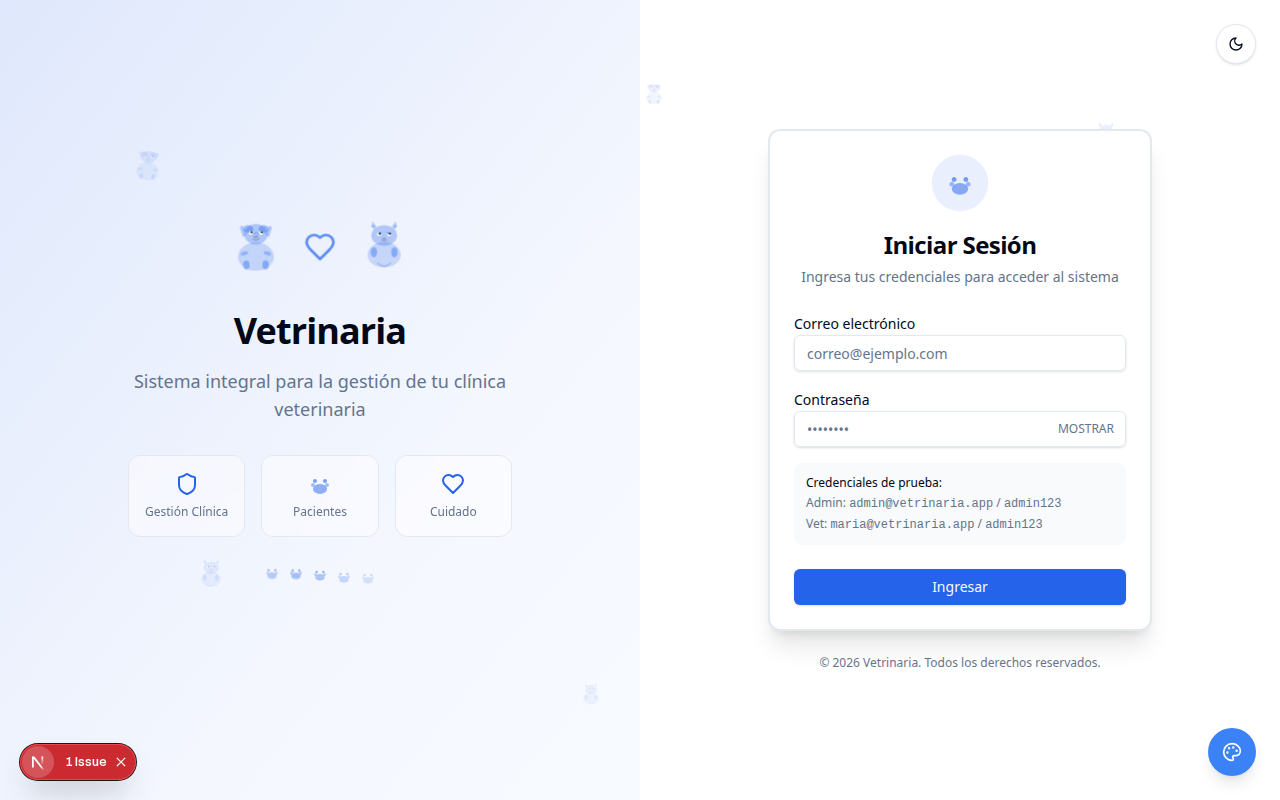
\includegraphics[width=0.8\textwidth]{img/vet-login.png}
    \caption{Pantalla de inicio de sesion con animaciones Framer Motion}
    \label{fig:login}
\end{figure}
